\section{Simulation}
Algorithm 1 shows the pseudo code for the simulation of Lévy process. The original code is covered in the appendix. 
\iffalse
\begin{figure}[H]
    \hrule
    \vspace*{0.2cm}
    \begin{enumerate}
    \item $\lambda_1, \lambda_2, \mu, \sigma \xleftarrow{} 1$. $\phi_{1}=-\frac{\mu}{\sigma^{2}}+\sqrt{\frac{\mu^{2}}{\sigma^{4}}+\frac{2 \lambda_1}{\sigma^{2}}}$, $\phi_{2}=\frac{\mu}{\sigma^{2}}+\sqrt{\frac{\mu^{2}}{\sigma^{4}}+\frac{2 \lambda_1}{\sigma^{2}}}$. F$\leftarrow{}$exp($\lambda_2$). $N_{loop} \leftarrow{}$ 100, $N_{jump} \leftarrow{}$ 1000. $A_{1000},M_{1000},P_{1000}\xleftarrow{}\Vec{0}_{N_{loop}}$
    \item $i\leftarrow{}1$. Initialize: $S, T, A, M, P, V, W, Y\xleftarrow{}\Vec{0}_{N_{jump}+1}$
    \item $j\leftarrow{}1$. Generate variables: $T_j \sim exp(\lambda_1)$, $V_j \sim exp(\phi_1$, $W_j \sim exp(\phi_2)$, $Y_j \sim exp(\lambda_2)$ 
    \item $S_j\leftarrow{}S_{j-1}+T_j$, $P_{j}\leftarrow{}A_{j-1}+\left(V_{j}-W_{j}\right)$, $A_{j}\leftarrow{}A_{j-1}+\left(V_{j}-W_{j}\right)+Y_{j}$,   $M_{j}\leftarrow{}\max \left\{M_{j-1}, A_{j-1}+V_{j}, A_{j-1}+\left(V_{j}-W_{j}\right)+Y_{j}\right\}$.
    \item $j\leftarrow{}j+1$, return to step 3 while $j \leq N_{jump}$
    \item  $A_{1000}(i)\leftarrow{}A(end),M_{1000}(i)\leftarrow{}M(end),P_{1000}(i)\leftarrow{}P(end)$
    \item $i\leftarrow{}i+1$, return to step 2 while $i \leq N_{loop}$
    \end{enumerate}
    \vspace*{0.2cm}
    \hrule
    \vspace*{0.2cm}
    \caption{Pseudo code for the simulation algorithm}
    \label{fig:step1}
\end{figure}
\fi

\begin{algorithm}[H]
\SetAlgoLined
\KwResult{$A_{i,j}$, $M_{i,j}$, $P_{i,j}$, $S_{i,j}$}
 Initialization:
 $\lambda_1, \lambda_2, \mu, \sigma \leftarrow{} 1$
 
 $\phi_{1}=-\frac{\mu}{\sigma^{2}}+\sqrt{\frac{\mu^{2}}{\sigma^{4}}+\frac{2 \lambda_1}{\sigma^{2}}}$

 $\phi_{2}=\frac{\mu}{\sigma^{2}}+\sqrt{\frac{\mu^{2}}{\sigma^{4}}+\frac{2 \lambda_1}{\sigma^{2}}}$.

 $N_{paths} \leftarrow{} 100$
 
 $N_{jumps} \leftarrow{} 1000$. 
 
 $A_{0,0},M_{0,0},P_{0,0}, S_{0,0}\xleftarrow{}0$
 
 $i \leftarrow{0}$, $j\leftarrow{1}$
 
 \While{i \le N_{loop} - 1 }
 {
  \While{j \le N_{jump}}
  {
  \text{Generate variates:} $T_{i,j} \sim exp(\lambda_1)$, $V_{i,j} \sim exp(\phi_1$), $W_{i,j} \sim exp(\phi_2)$, $Y_{i,j} \sim exp(\lambda_2)$
  
  $S_{i,j}\leftarrow{}S_{i,j-1}+T_{i,j}$
  
  $P_{i,j}\leftarrow{}A_{i,j-1}+\left(V_{i,j}-W_{i,j}\right)$
  
  $A_{i,j}\leftarrow{}A_{i,j-1}+\left(V_{i,j}-W_{i,j}\right)+Y_{i,j}$
  
  $M_{i,j}\leftarrow{}\max \left\{M_{i,j-1}, A_{i,j-1}+V_{i,j}, A_{i,j-1}+\left(V_{i,j}-W_{i,j}\right)+Y_{i,j}\right\}$.
  
  $j \leftarrow{j + 1}$
  
  }
  
  $i \leftarrow{i + 1}$
  
 }
 \caption{Simulation of the Lévy process}
\end{algorithm}



For a single 1000-jump process, the distribution of the final states of the Lévy process, (i.e. $\left(P_{1000}, A_{1000}, M_{1000}\right)$) are shown in the follows, where $\lambda_1, \lambda_2, \lambda_3, \mu, \sigma$ are all set to 1.

\begin{figure}[H]
\minipage{0.32\textwidth}
  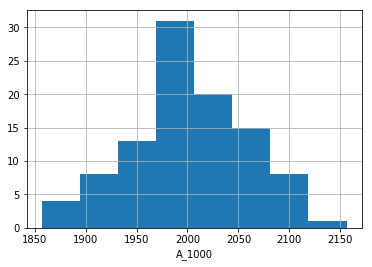
\includegraphics[width=\linewidth]{figures/task1-A.png}
  \caption{$A_{1000}$ for 100 runs}\label{fig:task1A}
\endminipage\hfill
\minipage{0.32\textwidth}
  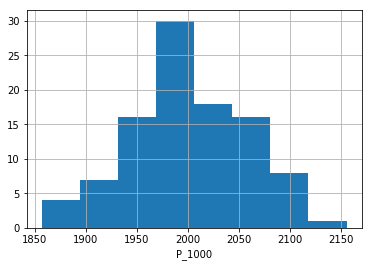
\includegraphics[width=\linewidth]{figures/task1-P.png}
  \caption{$P_{1000}$ for 100 runs}\label{fig:task1P}
\endminipage\hfill
\minipage{0.32\textwidth}%
  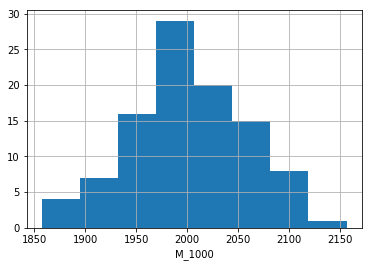
\includegraphics[width=\linewidth]{figures/task1-M.png}
  \caption{$M_{1000}$ for 100 runs}\label{fig:task1M}
\endminipage
\end{figure}


According to law of large numbers (LLN), $A_{1000}, P_{1000}, M_{1000}$ should satisfy normal distributions since each step in Lévy process can be considered as a reiterative trial, with means as:

For A,  
\begin{eqnarray*}
\mu_A& = &1000\mu_Y + 1000\mu_V - 1000\mu_W\\
&=&\frac{1000}{\lambda_2} + \frac{1000}{-\frac{\mu}{\sigma^{2}}+\sqrt{\frac{\mu^{2}}{\sigma^{4}}+\frac{2 \lambda_1}{\sigma^{2}}}} - \frac{1000}{\frac{\mu}{\sigma^{2}}+\sqrt{\frac{\mu^{2}}{\sigma^{4}}+\frac{2 \lambda_1}{\sigma^{2}}}} \\
&=&1000(1+\frac{1}{\sqrt{3}-1}-\frac{1}{\sqrt{3}+1}) = 2000
\end{eqnarray*}
It is similar to compute that 
$$\mu_P = 999\mu_Y + 1000\mu_V - 1000\mu_W = 1999$$


The 100 test results are summarized in table \ref{tab:task1}.
\begin{table}[h]
    \centering
        \caption{Mean and variance of different coordinates}
    \begin{tabular}{cccc}
    \hline
      Parameter   & Mean & Variance &Standard Deviation\\ \hline
       $A_{1000}$  & 2002.15&3312.29 & 57.84\\
       $P_{1000}$  & 2001.26 & 3324.44 & 57.95\\
       $M_{1000}$ & 2002.30 & 3313.83 & 57.86\\
       \hline
    \end{tabular}
    \label{tab:task1}
\end{table}

\newpage